\documentclass[preview,border=2pt]{standalone}
% Deployed lifecycle (mainline code base, 2026-11-06): release accepted on the
% force-balance score gamma_acc (arm D), opened by the release command or by the
% airborne-load watchdog.  Derived from fig_lifecycle_fsm_massonly.tex (cohort).
% Build: pdflatex fig_lifecycle_fsm_deployed.tex
\usepackage{times}
\usepackage{amsmath,amssymb,bm}
\usepackage{siunitx}
\usepackage{tikz}
\usetikzlibrary{arrows.meta,positioning,fit,backgrounds,calc}
\DeclareTextFontCommand{\textsc}{\upshape\scshape}
\begin{document}
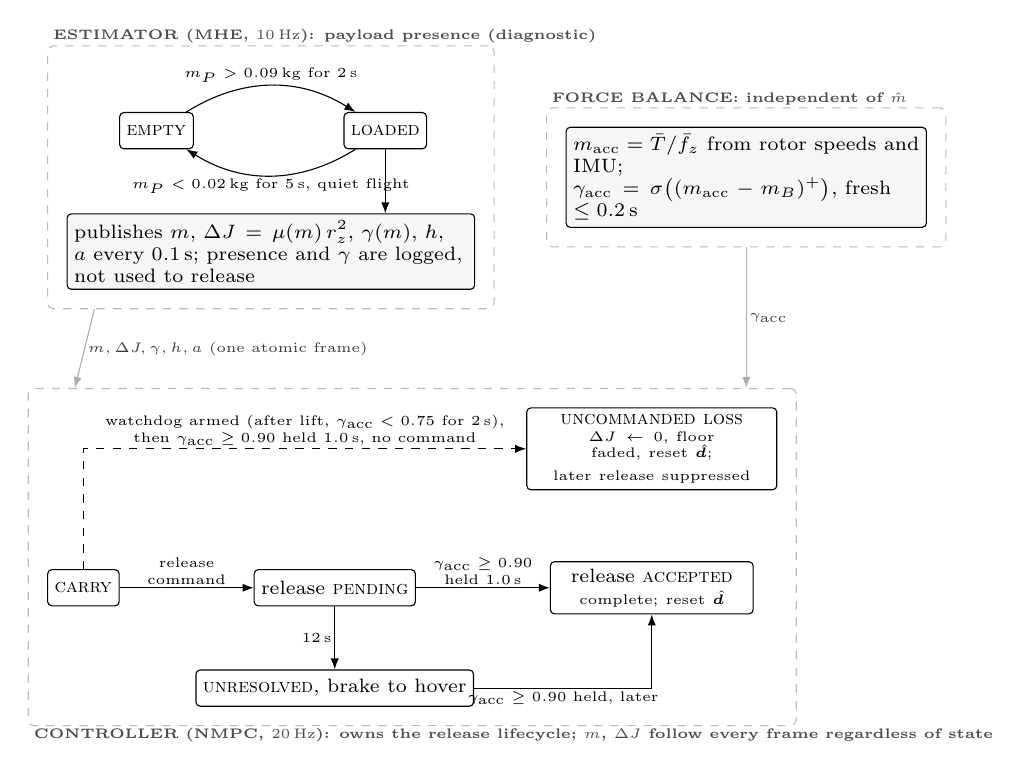
\begin{tikzpicture}[
  st/.style={draw,rounded corners=1.5pt,align=center,inner sep=2.5pt,
             minimum height=4.6mm,font=\scriptsize},
  ar/.style={-{Latex[length=1.4mm]},thin},
  lb/.style={font=\tiny,align=center,inner sep=1pt},
  lane/.style={draw=gray!55,dashed,rounded corners=2pt,inner sep=2.4mm},
  hd/.style={font=\tiny\bfseries,text=gray!60!black,inner sep=0.6pt},
]
% ============ estimator lane ============
\node[st] (empty) {\textsc{empty}};
\node[st,right=19mm of empty] (loaded) {\textsc{loaded}};
\draw[ar] (empty) to[out=32,in=148]
  node[lb,above,pos=.5] (lab1) {$m_P>\SI{0.09}{kg}$ for \SI{2}{s}} (loaded);
\draw[ar] (loaded) to[out=212,in=-32]
  node[lb,below,pos=.5] (lab2) {$m_P<\SI{0.02}{kg}$ for \SI{5}{s}, quiet flight} (empty);
\node[st,below=10.5mm of $(empty)!0.5!(loaded)$,fill=gray!7,text width=50mm,align=left]
  (ref) {\scriptsize publishes $m$, $\Delta J=\mu(m)\,r_z^2$, $\gamma(m)$, $h$, $a$
         every \SI{0.1}{s}; presence and $\gamma$ are logged, not used to release};
\draw[ar] (loaded.south) -- (loaded.south|-ref.north);
\begin{scope}[on background layer]
  \node[lane,fit=(empty)(loaded)(ref)(lab1)(lab2)] (elane) {};
\end{scope}
\node[hd,anchor=south west] at ([xshift=0.5mm]elane.north west)
  {ESTIMATOR (MHE, \SI{10}{Hz}): payload presence (diagnostic)};
% ============ force-balance evidence (inside the controller) ============
\node[st,right=9mm of elane.east,anchor=west,fill=gray!7,text width=44mm,align=left]
  (fb) {\scriptsize $m_{\mathrm{acc}}=\bar T/\bar f_z$ from rotor speeds and IMU;\\
        $\gamma_{\mathrm{acc}}=\sigma\bigl((m_{\mathrm{acc}}-m_B)^{+}\bigr)$, fresh $\le\SI{0.2}{s}$};
\begin{scope}[on background layer]
  \node[lane,fit=(fb)] (flane) {};
\end{scope}
\node[hd,anchor=south west] at ([xshift=0.5mm]flane.north west)
  {FORCE BALANCE: independent of $\hat m$};
% ============ controller lane: release lifecycle ============
\node[st,below=33mm of elane.south west,anchor=north west] (carry) {\scriptsize\textsc{carry}};
\node[st,right=17mm of carry] (pend) {\scriptsize release \textsc{pending}};
\node[st,right=17mm of pend,text width=24mm] (acc) {\scriptsize release \textsc{accepted}\\ \tiny complete; reset $\hat{\bm d}$};
\node[st,below=8mm of pend] (unres) {\scriptsize\textsc{unresolved}, brake to hover};
\node[st,above=9mm of acc,text width=30mm] (loss) {\scriptsize \textsc{uncommanded loss}\\
  \tiny $\Delta J\!\leftarrow\!0$, floor faded, reset $\hat{\bm d}$;\\ \tiny later release suppressed};
\draw[ar] (carry) -- node[lb,above,pos=.5] (lab4) {release\\command} (pend);
\draw[ar] (pend) -- node[lb,above,pos=.5] (lab3) {$\gamma_{\mathrm{acc}}\ge0.90$\\held \SI{1.0}{s}} (acc);
\draw[ar] (pend) -- node[lb,left,pos=.5] {\SI{12}{s}} (unres);
\draw[ar] (unres.east) -| node[lb,below,pos=.25] {$\gamma_{\mathrm{acc}}\ge0.90$ held, later} (acc.south);
\draw[ar,dashed] (carry.north) |- node[lb,above,pos=.75] (lab5)
  {watchdog armed (after lift, $\gamma_{\mathrm{acc}}<0.75$ for \SI{2}{s}),\\
   then $\gamma_{\mathrm{acc}}\ge0.90$ held \SI{1.0}{s}, no command} (loss.west);
\begin{scope}[on background layer]
  \node[lane,fit=(carry)(pend)(acc)(unres)(loss)(lab3)(lab4)(lab5)] (clane) {};
\end{scope}
\node[hd,anchor=north west] at ([xshift=0.5mm]clane.south west)
  {CONTROLLER (NMPC, \SI{20}{Hz}): owns the release lifecycle; $m$, $\Delta J$ follow every frame regardless of state};
\draw[ar,gray!65] ([xshift=6mm]elane.south west) -- ([xshift=6mm]clane.north west)
  node[lb,right,pos=.5,text=gray!45!black] {$m,\Delta J,\gamma,h,a$ (one atomic frame)};
\draw[ar,gray!65] (flane.south) -- (flane.south|-clane.north)
  node[lb,right,pos=.5,text=gray!45!black] {$\gamma_{\mathrm{acc}}$};
\end{tikzpicture}
\end{document}
